\documentclass{mp}
\graphicspath{{13_lancuchy_markowa}}
\subtitle{Łańcuchy Markowa}
\usetikzlibrary{automata}
\begin{document}
\frame{\titlepage}
\begin{frame}{Łańcuch Markowa}
\[ \{X_t,T\} \]
\begin{itemize}
\item $T=\{0,1,2,\ldots\}$
\item $P(X_t\in\{x_0,x_1,\ldots,x_n,\ldots\})=1$
\item $\{X_t\}$ jest procesem Markowa
\item \[\forall x_i,x_j,t\colon P(X_t=x_j|X_{t-1}=x_i)=P_{i,j}\]
\end{itemize}
\end{frame}
\begin{frame}{Macierz przejść}
\begin{gather*}
\bm{P}=\begin{bmatrix} 
P_{0,0} & P_{0,1} & \ldots & P_{0,j} & \ldots \\
P_{1,0} & P_{1,1} & \ldots & P_{1,j} & \ldots \\
\vdots & \vdots & \ddots & \vdots & \ddots \\
P_{i,0} & P_{i,1} & \ldots & P_{i,j} & \ldots \\
\vdots & \vdots & \ddots & \vdots & \ddots \\
\end{bmatrix} \\
\bm{P(X_t)}=\begin{bmatrix} P(X_t=a_1) & P(X_t=a_2) & \ldots & P(X_t=a_j) & \ldots \end{bmatrix} \\
\uncover<2->{\bm{P(X_t)}\bm{P}=\alert<2>{?}\\}
\uncover<3->{\bm{P(X_t)}\bm{P^k}=\alert<3>{?}}
\end{gather*}
\note<2>{
	Ile wynoszą sumy w wierszach w macierzy? \\
	$\bm{P(X_t)}\bm{P}=\bm{P(X_{t+1})}$}
\end{frame}
\begin{frame}{Kolejka w routerze}
\center
\begin{tikzpicture}[
	packet1/.style={draw=black,fill=color2},
	packet2/.style={draw=black,fill=color3},
	packet3/.style={draw=black,fill=color4},
	]
\node (router) {\includegraphics[width=2cm]{13_lancuchy_markowa/router.png}};
\node (s1) [draw,thick,color2,above left=of router] {\includegraphics[width=1.5cm]{13_lancuchy_markowa/server.png}};
\node (s2) [draw,thick,color3,below left=of router] {\includegraphics[width=1.5cm]{13_lancuchy_markowa/server.png}};
\node (s3) [draw,thick,color4,right=of router] {\includegraphics[width=1.5cm]{13_lancuchy_markowa/server.png}};
\draw (s1) -- (router);
\draw (s2) -- (router);
\draw (s3) -- (router);
\filldraw[visible on=<1>,packet1] ($.5*(router)+.5*(s1)+(-.25cm,-.25cm)$) rectangle ++(.5cm,.5cm);
\filldraw[visible on=<2>,packet1] ($(router)+(-.25cm,-.25cm)$) rectangle ++(.5cm,.5cm);
\filldraw[visible on=<3>,packet1] ($.5*(router)+.5*(s2)+(-.25cm,-.25cm)$) rectangle ++(.5cm,.5cm);
\begin{scope}[visible on=<4>]
\filldraw[packet1] ($.5*(router)+.5*(s1)+(-.25cm,-.25cm)$) rectangle ++(.5cm,.5cm);
\filldraw[packet1] ($.4*(router)+.6*(s1)+(-.25cm,-.25cm)$) rectangle ++(.5cm,.5cm);
\filldraw[packet2] ($.5*(router)+.5*(s2)+(-.25cm,-.25cm)$) rectangle ++(.5cm,.5cm);
\filldraw[packet2] ($.4*(router)+.6*(s2)+(-.25cm,-.25cm)$) rectangle ++(.5cm,.5cm);
\filldraw[packet3] ($.5*(router)+.5*(s3)+(-.25cm,-.25cm)$) rectangle ++(.5cm,.5cm);
\filldraw[packet3] ($.4*(router)+.6*(s3)+(-.25cm,-.25cm)$) rectangle ++(.5cm,.5cm);
\end{scope}
\begin{scope}[visible on=<5-6>]
\filldraw[packet1] ($(router)+(-.4cm,0)+(-.25cm,-.25cm)$) rectangle ++(.5cm,.5cm);
\filldraw[packet1] ($(router)+(-.2cm,0)+(-.25cm,-.25cm)$) rectangle ++(.5cm,.5cm);
\filldraw[packet2] ($(router)+(0,0)+(-.25cm,-.25cm)$) rectangle ++(.5cm,.5cm);
\filldraw[packet2] ($(router)+(.2cm,0)+(-.25cm,-.25cm)$) rectangle ++(.5cm,.5cm);
\filldraw[packet3] ($(router)+(.4cm,0)+(-.25cm,-.25cm)$) rectangle ++(.5cm,.5cm);
\begin{scope}[visible on=<6>]
\node (trash) [below=of router] {
\includegraphics[width=1.5cm]{13_lancuchy_markowa/garbage.png}};
\filldraw[packet3] ($(trash)+(0,.5cm)+(-.25cm,-.25cm)$) rectangle ++(.5cm,.5cm);
\end{scope}
\end{scope}
\end{tikzpicture}
\tiny{Rysunki z domeny publicznej, \url{http://pixbay.com}, użytkownik \emph{Nemo}}
\end{frame}
\begin{frame}{Model kolejki w routerze (\texttt{M|M|1|5})}
\only<-4>
{
\center
\begin{tikzpicture}[every state/.style={circle}]
\node (n0) [state] {0};
\node (n1) [state,right=of n0] {1};
\node (n2) [state,right=of n1] {2};
\node (n3) [state,right=of n2] {3};
\node (n4) [state,right=of n3] {4};
\node (n5) [state,right=of n4] {5};
\foreach \src/\dst in {n0/n1,n1/n2,n2/n3,n3/n4,n4/n5}
{
	\path[->] (\src) edge[bend left] node[above] {$0{,}1$} (\dst);
	\path[->] (\dst) edge[bend left] node[below] {$0{,}2$} (\src);
}
\path[->] (n0) edge[loop above] node[above] {$0{,}9$} (n0);
\foreach \n in {n1,n2,n3,n4}
	\path[->] (\n) edge[loop above] node[above] {$0{,}7$} (\n);
\path[->] (n5) edge[loop above] node[above] {$0{,}8$} (n5);
\end{tikzpicture}
}
\only<5->
{
	\begin{align*}
	 \bm{P}(X_0) & = \begin{bmatrix} 0{,}10 & 0{,}10 & 0{,}15 & 0{,}25 & 0{,}25 & 0{,}15 \end{bmatrix}  \\
	 \uncover<6->{\bm{P}(X_0)\bm{P}^{10} & = \begin{bmatrix} 0{,}23 &  0{,}18 &  0{,}18 &  0{,}17 &  0{,}14 &  0{,}09 \end{bmatrix}}
	\end{align*}
}
\uncover<2->
{
\begin{columns}[T]
\begin{column}{.49\textwidth}
\tabcolsep=.8\tabcolsep
\begin{tabular}{l|llllll}
$\bm{P}$ & 0 & 1 & 2 & 3 & 4 & 5 \\
\hline
0 & $0{,}9$ & $0{,}1$ &  &  &  &  \\
1 & $0{,}2$ & $0{,}7$ & $0{,}1$ &  &  &  \\
2 &  & $0{,}2$ & $0{,}7$ & $0{,}1$ &  &  \\
3 &  &  & $0{,}2$ & $0{,}7$ & $0{,}1$ &  \\
4 &  &  &  & $0{,}2$ & $0{,}7$ & $0{,}1$ \\
5 &  &  &  &  & $0{,}2$ & $0{,}8$  \\
\end{tabular}
\end{column}
\begin{column}{.49\textwidth}
\uncover<3->
{
\tabcolsep=.5\tabcolsep
\only<3>
{
\begin{tabular}{l|llllll}
$\alert{\bm{P}^2}$ & 0 & 1 & 2 & 3 & 4 & 5 \\
\hline
0 & $0{,}83$ & $0{,}16$ & $0{,}01$ &  &  & \\
1 & $0{,}32$ & $0{,}53$ & $0{,}14$ & $0{,}01$ &  &  \\
2 & $0{,}04$ & $0{,}28$ & $0{,}53$ & $0{,}14$ & $0{,}01$ & \\
3 &  & $0{,}04$ & $0{,}28$ & $0{,}53$ & $0{,}14$ & $0{,}01$ \\
4 &  &  & $0{,}04$ & $0{,}28$ & $0{,}53$ & $0{,}15$ \\
5 &  &  &  & $0{,}04$ & $0{,}30$ & $0{,}66$
\end{tabular}
}
\only<4->
{
\begin{tabular}{l|llllll}
$\alert<4>{\bm{P}^{10}}$ & 0 & 1 & 2 & 3 & 4 & 5\\
\hline
 0 &  $0{,}63$ & $0{,}26$ & $0{,}09$ & $0{,}02$ &  &  \\
 1 &  $0{,}52$ & $0{,}27$ & $0{,}13$ & $0{,}05$ & $0{,}01$ &  \\
 2 &  $0{,}35$ & $0{,}27$ & $0{,}20$ & $0{,}12$ & $0{,}05$ & $0{,}02$ \\
 3 &  $0{,}18$ & $0{,}20$ & $0{,}24$ & $0{,}20$ & $0{,}12$ & $0{,}06$ \\
 4 &  $0{,}07$ & $0{,}12$ & $0{,}20$ & $0{,}25$ & $0{,}22$ & $0{,}15$ \\
 5 &  $0{,}02$ & $0{,}06$ & $0{,}14$ & $0{,}24$ & $0{,}30$ & $0{,}25$ \\
\end{tabular}
}
}
\end{column}
\end{columns}
}
\end{frame}
\begin{frame}{Klasyfikacja stanów}
\note<1>{
	$r_{i,j}^t$ prawdopodobieństwo, że przejdziemy z $x_i$ do $x_j$ w dokładnie $t$ krokach.
	Nie tworzy zmiennej losowej, bo nie musi się sumować do 1. \\
	$h_{i,j}$ to średni czas przejścia $i\to j$. \\
	Do stanu powracającego łańcuch wraca nieskończenie wiele razy \\
	Stany zerowe powracające nie mogą występować w łańcuchach skończonych.
}
\begin{gather*}
 r_{i,j}^t=P\left(X_t=x_j, X_{t-1}\neq x_j, X_{t-2}\neq x_j, \ldots, X_1\neq x_j,  | X_0=x_i\right) \\
 h_{i,j}=\sum_{t=1}^\infty tr_{i,j}^t
\end{gather*}
\only<2>
{
\begin{description}
\item[dodatni powracający] \[\sum_{t=1}^\infty r_{i,i}^t =1 \land h_{i,i}<\infty\]
\item[zerowy powracający] \[\sum_{t=1}^\infty r_{i,i}^t =1 \land h_{i,i}=\infty\]
\item[przejściowy] \[\sum_{t=1}^\infty r_{i,i}^t <1 \]
\end{description}
}
\only<3->
{
\begin{block}{Przykład}
\center
\begin{tikzpicture}
\node (n1) [state] {1};
\node (n2) [state,right=of n1] {2};
\node (n3) [state,right=of n2] {3};
\node (dots1) [right=of n3] {\ldots};
\node (abovedots1) [above=of dots1] {};
\node (nn) [state,right=of dots1] {n};
\node (dots2) [right=of nn] {\ldots};


\path[->] (n1) edge[bend left] node[above] {$\frac{1}{2}$} (n2);
\path[->] (n1) edge[loop below] node[below] {$\frac{1}{2}$} (n1);
\path[->] (n2) edge[bend left] node[above] {$\frac{2}{3}$} (n3);
\path[->] (n2) edge[bend left] node[below] {$\frac{1}{3}$} (n1);
\path[->] (n3) edge[bend left] node[below] {$\frac{1}{4}$} (n1);
\path[->] (n3) edge[bend left] node[above] {$\frac{3}{4}$} (dots1);
\path[->] (dots1) edge[bend left] node[above] {$\frac{n-1}{n}$} (nn);
\path[->] (nn) edge[bend left] node[above] {$\frac{n}{n+1}$} (dots2);
\path[->] (nn) edge[bend left] node[below] {$\frac{1}{n+1}$} (n1);
\end{tikzpicture}
\note<3>
{
\begin{gather*}
r_{1,1}^t=\prod_{j=1}^{t-1} \frac{j}{j+1}\cdot\frac{1}{t+1}=\frac{1}{2}\cdot\frac{2}{3}\cdot\ldots\cdot\frac{t-1}{t}\cdot\frac{1}{t+1}=\frac{1}{t(t+1)} \\
\sum_{t=1}^\infty \frac{1}{t(t+1)}=\lim_{n\to\infty} \frac{n}{n+1}=1 \\
h_{i,i}=\sum_{t=1}^\infty \frac{t}{t(t+1)}=\sum_{t=1}^\infty \frac{1}{t+1}=\infty
\end{gather*}
}
\begin{gather*}
\uncover<4->{r_{1,1}^t=\alert<4>{?} \qquad}
\uncover<5->{\sum_{t=1}^\infty r_{1,1}^t=\alert<5>{?} \qquad}
\uncover<6->{h_{1,1}^t=\alert<6>{?}}
\end{gather*}
\end{block}
}
\end{frame}
\begin{frame}{Okresowość łańcucha}
\note<1>{Łańcuch jest okresowy jeżeli którykolwiek ze stanów jest okresowy}
\begin{block}{Stan okresowy $x_j$}
\begin{gather*}
 \exists \Delta\in\{2,3,\ldots\} \forall t,t+s\in T\colon \\ \left( P(X_{t+s}=x_j|X_t=x_j)=0 \iff s\mod\Delta\neq 0\right) 
\end{gather*}
\end{block}
\only<2>{\alert{Czy łańcuch z poprzedniego slajdu jest okresowy?}}
\only<3>
{
\begin{block}{Inny przykład}
\begin{tikzpicture}
\node (n1) [state] {0};
\node (n2) [state,right=of n1] {1};
\node (n3) [state,right=of n2] {2};
\node (dots1) [right=of n3] {\ldots};
\node (abovedots1) [above=of dots1] {};
\node (nn) [state,right=of dots1] {n};
\node (dots2) [right=of nn] {\ldots};

\path[->] (n1) edge[bend left] node[above] {$1$} (n2);
\path[->] (n2) edge[bend left] node[above] {$\frac{1}{2}$} (n3);
\path[->] (n3) edge[bend left] node[above] {$\frac{2}{3}$} (dots1);
\path[->] (dots1) edge[bend left] node[above] {$\frac{n-1}{n}$} (nn);
\path[->] (nn) edge[bend left] node[above] {$\frac{n}{n+1}$} (dots2);

\path[->] (n2) edge[bend left] node[below] {$\frac{1}{2}$} (n1);
\path[->] (n3) edge[bend left] node[below] {$\frac{1}{3}$} (n2);
\path[->] (dots1) edge[bend left] node[below] {$\frac{1}{4}$} (n3);
\path[->] (nn) edge[bend left] node[below] {$\frac{1}{n+1}$} (dots1);
\path[->] (dots2) edge[bend left] node[below] {$\frac{1}{n+2}$} (nn);



% \path[->] (n1) edge[bend left] node[above] {$1$} (n2);
% \path[->] (n2) edge[bend left] node[above] {$\frac{1}{2}$} (n3);
% \path[->] (n2) edge[bend left] node[below] {$\frac{1}{2}$} (n1);
% \path[->] (n3) edge[bend left] node[below] {$\frac{1}{2}$} (n2);
% \path[->] (n3) edge[bend left] node[above] {$\frac{1}{2}$} (dots1);
% \path[->] (dots1) edge[bend left] node[below] {$\frac{1}{2}$} (n3);
% \path[->] (dots1) edge[bend left] node[above] {$\frac{1}{2}$} (nn);
% \path[->] (dots2) edge[bend left] node[below] {$\frac{1}{2}$} (nn);
% \path[->] (nn) edge[bend left] node[above] {$\frac{1}{2}$} (dots2);
% \path[->] (nn) edge[bend left] node[below] {$\frac{1}{2}$} (dots1);

\end{tikzpicture}
\end{block}
}
\end{frame}
\begin{frame}{Rozkład stacjonarny $\bm{\pi}$}
\note<1>{$\bm{\pi}$ ma być rozkładem prawdopodobieństwa, więc nieujemne i sumować się do 1.}
\[ \bm{\pi}\bm{P}=\bm{\pi} \]
\uncover<2->
{
\begin{block}{Wniosek}
\begin{enumerate}
\item Jeżeli dla pewnego $N\in T$ zachodzi $\forall x_i\colon P(X_N=x_i)=\pi_i$, to
\[ \forall n>N\forall x_i\colon P(X_n=x_i)=\pi_i \]
\uncover<3->{\item Jeżeli $\forall x_i\colon P(X_0=x_i)=\pi_i$, to $\{X_t\}$ jest stacjonarny w węższym sensie.}
\end{enumerate}
}
\end{block}
\end{frame}
\begin{frame}{Nieredukowalność}
%na podstawie P:TE Theorem 6.4.5
\note<1>{Jeżeli łańcuch nie jest nieredukowalny, to można zastosować twierdzenie o rozkładaniu (ang. \emph{Decomposition theorem}) i rozłożyć go na odrębne, nieredukowalne fragmenty plus stany przejściowe, które w analizie stacjonarności nie mają znaczenia.}
\begin{block}{Określenie}
\[ \forall x_i,x_j \exists t\in T \colon (\bm{P}^t)_{i,j}>0 \]
\end{block}
\only<2-5>
{
	\note<5>{$\{1,2\}$ są nieredukowalne i dodatnie powracające, $\{3,4\}$ są przejściowe, a $\{5, \ldots\}$ są nieredukowalne, ale zerowo powracające. $\{3,4\}$ mają zerowe rozkłady stacjonarne, obliczenie rozkładu stacjonarnego $\{1,2\}$ nie zależy od rozkładów stacjonarnych $\{5,\ldots\}$ (i vice-versa).}
\begin{block}{Oblicz rozkład stacjonarny}
\begin{tikzpicture}
\node (empty) {};
\node (n1) [state,left=of empty] {1};
\node (n2) [state,below=of n1] {2};

\path[->] (n1) edge[loop above] node[above] {$0{,}1$} (n1);
\path[->] (n1) edge[bend left] node[right] {$0{,}9$} (n2);
\path[->] (n2) edge[bend left] node[left] {$0{,}9$} (n1);
\path[->] (n2) edge[loop below] node[below] {$0{,}1$} (n2);

\begin{scope}[visible on=<3->]
\node (n3) [state,right=of empty] {3};
\node (n4) [state,below=of n3] {4};
\path[->] (n3) edge[loop above] node[above] {$0{,}1$} (n3);
\path[->] (n3) edge[bend left] node[right] {\alt<-3>{$0{,}9$}{\alert<4>{$0{,}8$}}} (n4);
\path[->] (n4) edge[bend left] node[left] {\alt<-4>{$0{,}9$}{\alert<5>{$0{,}8$}}} (n3);
\path[->] (n4) edge[loop below] node[below] {$0{,}1$} (n4);
\path[->,visible on=<4->] (n3) edge[bend right] node[above] {\alert<4>{$0{,}1$}} (n1);
\end{scope}
\begin{scope}[visible on=<5->]
\node (n5) [state,right=of n4] {5};
\node (n6) [state,right=of n5] {6};
\node (dots1) [right=of n6] {\ldots};
\node (nn) [state,above=of dots1] {$n+4$};
\node (dots2) [above=of n5] {\ldots};

\path[->] (n4) edge[bend right] node[below] {$0{,}1$} (n5);
\path[->] (n5) edge[loop below] node[below] {$\frac{1}{2}$} (n5);
\path[->] (n5) edge[bend right] node[below] {$\frac{1}{2}$} (n6);
\path[->] (n6) edge[bend right] node[below] {$\frac{2}{3}$} (dots1);
\path[->] (n6) edge[bend right] node[above] {$\frac{1}{3}$} (n5);
\path[->] (dots1) edge[bend right] node[left] {$\frac{n-1}{n}$} (nn);
\path[->] (nn) edge[bend right] node[above] {$\frac{n}{n+1}$} (dots2);
\path[->] (nn) edge[bend right] node[above] {$\frac{1}{n+1}$} (n5);
\end{scope}
\end{tikzpicture}
\end{block}
}
\only<6->
{
	%Twierdzenie 7.11 u Mitzenmachera
	\note<6>{$\pi_i$ nie zależą od $x_j$, po prostu są równe niezależnie od wybranej wartości $j$.}
\begin{block}{Twierdzenie}
Jeżeli $\{X_t\}$ jest nieredukowalny, nieokresowy i wszstkie jego stany są dodatnie powracające, to \[\forall x_i,x_j\colon \pi_i=\lim_{t\to\infty} (\bm{P}^t)_{i,j}=\frac{1}{h_{i,i}} \]
\end{block}
}
\end{frame}
\begin{frame}{Uśrednianie po czasie}
%Example 7.2.2 w "Probability: theory and examples" R. Durret
\begin{block}{Twierdzenie ergodyczne}
Jeżeli $\{X_t\}$ jest nieredukowalny i ma rozkład stacjonarny, to dla dowolnej funkcji $f(X)$:
\[ \sum_{x_i} \left|f(x_i)\right|\pi_i<\infty \to P\left(\{\omega\colon \lim_{n\to\infty} \frac{1}{n}\sum_{t=0}^n f(X_t(\omega))=\sum_{x_i}f(x_i)\pi_i\}\right)=1\]
\end{block}
\begin{block}{Wniosek}
Dla stacjonarnego łańcucha Markowa o skończonej wartości średniej i wariancji oraz jego realizacji $(x_1,x_2,\ldots,x_n)$:
\[EX\approx \frac{1}{n}\sum_{t=0}^n x_t \qquad DX^2\approx \frac{1}{n}\sum_{t=0}^n x_t^2-E^2X \]
\end{block}
\end{frame}
\begin{frame}{Długa kolejka}
\only<1>
{
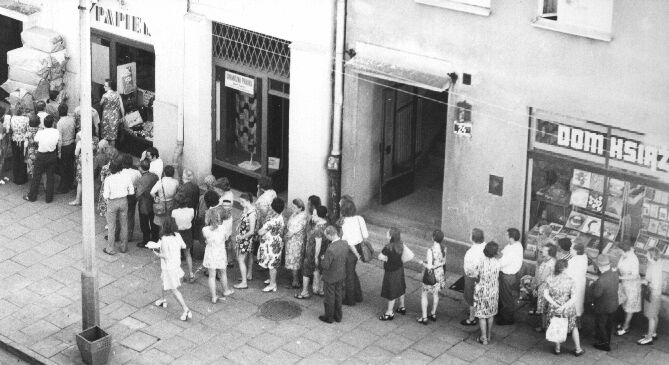
\includegraphics[width=\textwidth]{13_lancuchy_markowa/Kolejka.jpeg}

{\tiny \url{http://commons.wikimedia.org/wiki/File:Kolejka.jpeg} domena publiczna}
}
\only<2->
{
	\begin{block}{Dyskretna kolejka \texttt{M|M|1}}
	\center
		\begin{tikzpicture}[every state/.style={circle}]
		\node (n0) [state] {0};
	\node (n1) [state,right=of n0] {1};
	\node (n2) [state,right=of n1] {2};
	\node (dots1) [right=of n2] {\ldots};
	\node (nn) [state,right=of dots1] {n};
	\node (dots2) [right=of nn] {\ldots};
	\foreach \src/\dst in {n0/n1,n1/n2,n2/dots1,dots1/nn,nn/dots2}
	{
		\path[->] (\src) edge[bend left] node[above] {$\lambda$} (\dst);
		\path[->] (\dst) edge[bend left] node[below] {$\mu$} (\src);
	}
	\path[->] (n0) edge[loop above] node[above] {$1-\lambda$} (n0);
	\foreach \n in {n1,n2,nn}
	\path[->] (\n) edge[loop above] node[above] {$1-\mu-\lambda$} (\n);
	\end{tikzpicture}
	\end{block}
\uncover<3->
{
\begin{block}{Problemy}
\begin{enumerate}
\item $\bm{\pi}=\alert<3>{?}$
\item<4-> Niech $P(X_0)=\bm{\pi}$. $EX=\alert<4>{?}$
\item<5-> W przeciągu 10000000 kwantów czasu naliczono średnio 5 klientów w~kolejce. \alert<5>{Co z tego?}
\item<6-> Ile średnio czasu \alert<6>{czeka pojedynczy klient} jeżeli obsługujemy FIFO?
\end{enumerate}
\end{block}
}
\note<1>
{
	$\bm{\pi}$ liczymy z definicji, wychodzi $\pi_n=\varrho^n(1-\varrho)$, gdzie $\varrho=\frac{\lambda}{\mu}<1$.
	Skoro $P(X_t=n)=\varrho^n(1-\varrho)$ dla $n\in\N_0$, to $P(X_t+1=n)=\varrho^{n-1}(1-\varrho)$ dla $n\in\N_+$, a zatem $X_t+1$ ma rozkład geometryczny o parametrze $1-\varrho$ i w takim razie $E(X_t+1)=\frac{1}{1-\varrho}$.

	Odwołujemy się do twierdzenia ergodycznego i przybliżamy $EX_t=5$, a w takim razie $\varrho=1-\frac{1}{5+1}=\frac{5}{6}$.
}
\note<6>
{
	$W$ -- czas od momentu wejścia do systemu do momentu wyjścia, $X$ -- liczba klientów w systemie w momencie wejścia
	\[EW=\sum_{k=0}^\infty E(W|X=k)P(X=k)=\sum_{k=0}^\infty E(W|X=k)\pi_k \]
	Obsługiwany klient w każdym kwancie czasu z prawdopodobieństwem $\mu$ kończy być obsługiwany i opuszcza system, a z prawdopodobieństwem $1-\mu$ nadal jest obsługiwany. Zatem:
	\[ P(W=t|X=0)=(1-\mu)^{t-1}\mu \]
	czyli $W|X=0$ ma rozkład geometryczny z parametrem $\mu$, a~w~takim razie $E(W|X=0)=\frac{1}{\mu}$.
	Jeżeli w systemie jest $k$ klientów, a każdy jest obsługiwany niezależnie, to nowy klient musi przeczekać tych $k$ klientów i samemu zostać obsłużonym. Zatem $E(W|X=0)=\frac{k+1}{\mu}$ i:
	\[EW=\sum_{k=0}^\infty \frac{k+1}{\mu}\pi_k=\frac{1}{\mu}\left(\sum_{k=0}^\infty k\pi_k + \sum_{k=0}^\infty \pi_k\right) \]
	Pierwszy składnik sumy to wartość średnia liczby klientów w systemie ($EX$), a drugi składnik sumy z definicji jest równy 1, zatem
	\[EW=\frac{EX+1}{\mu}=\frac{\frac{\varrho}{1-\varrho}+1}{\mu}=\frac{1}{(1-\varrho)\mu}=\frac{1}{\mu-\lambda} \]
}
}
\end{frame}
\end{document}
